%% LyX 2.3.6.1 created this file.  For more info, see http://www.lyx.org/.
%% Do not edit unless you really know what you are doing.
\documentclass[english]{article}
\usepackage[T1]{fontenc}
\usepackage[latin9]{inputenc}
\usepackage{geometry}
\geometry{verbose,tmargin=2.5cm,bmargin=2.5cm,lmargin=2.5cm,rmargin=2.5cm}
\usepackage{calc}
\usepackage{graphicx}

\makeatletter

%%%%%%%%%%%%%%%%%%%%%%%%%%%%%% LyX specific LaTeX commands.
%% Because html converters don't know tabularnewline
\providecommand{\tabularnewline}{\\}

\makeatother

\usepackage{babel}
\begin{document}
{[}SPLIT\_HERE{]}
\begin{enumerate}
\item \textbf{{[}DHS/PRELIM/9597/2018/P1/Q1{]} }

The file \texttt{LOG.TXT} contains the access log entries of an organisation's
website from 0000 to 1800 hours on 1 August 2018.

The entries have the following format: 
\begin{enumerate}
\item[1.]  \textbf{host} (domain name or IP address) making the request.
\item[2.]  \textbf{timestamp} in the format \textquotedbl DAY MON DD HH:MM:SS
YYYY\textquotedbl , where \textbf{DAY} is the day of the week, \textbf{MON}
is the name of the month, \textbf{DD} is the day of the month, \textbf{HH:MM:SS}
is the time of day using a 24-hour clock, and \textbf{YYYY} is the
year. The timezone is -0400.
\item[3.]  \textbf{request} in quotes. 
\item[4.]  \textbf{HTTP reply status code}. 
\item[5.]  \textbf{bytes in the reply}.
\end{enumerate}

\subsection*{Task 1.1 }

Determine the top 5 hosts which accessed the website during this period,
in descending frequency order.

Sample output: 

\noindent %
\noindent\begin{minipage}[t]{1\columnwidth}%
\texttt{Top 5 hosts: }

\texttt{1 139.230.35.135 ~~~~~~~~~~~187}

\texttt{2 ns2.sharp.co.jp ~~~~~~~~~~95 }

\texttt{3 194.157.109.130 ~~~~~~~~~~62 }

\texttt{3 ix-dfw12-08.ix.netcom.com 62 }

\texttt{4 piweba1y.prodigy.com ~~~~~55 }

\texttt{5 205.163.36.61 ~~~~~~~~~~~~30}%
\end{minipage}

\subsection*{Evidence 1 }

Program code.\hfill{} {[}9{]}

\subsection*{Evidence 2 }

Screenshot. \hfill{}{[}1{]}

\subsection*{Task 1.2}

Determine the host which returned the largest reply size and the largest
reply size.

Sample output: 

\texttt{slip4086.sirius.com 12345}

\subsection*{Evidence 3 }

Program code.\hfill{} {[}4{]}

\subsection*{Evidence 4 }

Screenshot. \hfill{}{[}1{]}

{[}SPLIT\_HERE{]}
\item \textbf{{[}DHS/PRELIM/9597/2018/P1/Q2{]} }

A media access control (MAC) address is a unique identification code
hardwired to and used to identify individual devices on the network,
and is often expressed using hexadecimal notation eg. \texttt{4c:21:d0:15:e3:ea}.

\subsection*{Task 2.1 }

Using top down design, write iterative program code to convert a given
MAC address to decimal notation. For MAC address \texttt{4c:21:d0:15:e3:ea},
its converted decimal notation will be \texttt{76:33:208:21:227:234}.

\subsection*{Evidence 5 }

Program code. \hfill{}{[}4{]}

\subsection*{Evidence 6}

Screenshot.\hfill{} {[}1{]}

\subsection*{Task 2.2}

Write recursive program code to convert a given MAC address to decimal
notation. Use the same MAC address \texttt{4c:21:d0:15:e3:ea} to test
your program code.

\subsection*{Evidence 7 }

Program code.\hfill{} {[}4{]}

\subsection*{Evidence 8 }

Screenshot. \hfill{}{[}1{]}

\subsection*{Task 2.3 }

Write program code to perform input validation for a MAC address.
Test your program with suitable test data.

\subsection*{Evidence 9 }

Program code. \hfill{}{[}3{]}

\subsection*{Evidence 10 }

Screenshots. \hfill{}{[}2{]}

{[}SPLIT\_HERE{]}
\item \textbf{{[}DHS/PRELIM/9597/2018/P1/Q3{]} }

A blockchain is a linked list of blocks where each block has the following
structure:
\begin{center}
\begin{tabular}{|l|l|l|}
\hline 
\multicolumn{3}{|c|}{Class\texttt{: Block}}\tabularnewline
\hline 
\multicolumn{3}{|c|}{Attributes}\tabularnewline
\hline 
\texttt{\hspace{0.01\columnwidth}}Identifier & \texttt{\hspace{0.01\columnwidth}}Data Type & \texttt{\hspace{0.05\columnwidth}}Description\tabularnewline
\hline 
\texttt{Data} & \texttt{String} & Block data\tabularnewline
\hline 
\texttt{PrevHash} & \texttt{String} & Hash of previous block\tabularnewline
\hline 
\texttt{CurrHash} & \texttt{String} & Hash of \texttt{Data} and \texttt{PrevHash}\tabularnewline
\hline 
\texttt{Next} & \texttt{Integer} & The next block pointer\tabularnewline
\hline 
\end{tabular}
\par\end{center}

The structure of the blockchain is as follows:
\begin{center}
\begin{tabular}{|l|l|l|}
\hline 
\multicolumn{3}{|c|}{Class\texttt{: BlockChain}}\tabularnewline
\hline 
\multicolumn{3}{|c|}{Attributes}\tabularnewline
\hline 
\texttt{\hspace{0.01\columnwidth}}Identifier & \texttt{\hspace{0.01\columnwidth}}Data Type & \texttt{\hspace{0.05\columnwidth}}Description\tabularnewline
\hline 
\texttt{ChainData} & \texttt{Array{[}1:20{]} of Block} & An array used to store the 20 blocks.\tabularnewline
\hline 
\texttt{Start} & \texttt{Integer} & Index for the genesis block.\tabularnewline
\hline 
\texttt{NextFreeBlock} & \texttt{Integer} & Index for the next available empty block.\tabularnewline
\hline 
\end{tabular}
\par\end{center}

The initial value of \texttt{Start} is 1 and the initial value of
\texttt{NextFreeBlock} is 1.

The first block of the blockchain is called the genesis block and
its \texttt{PrevHash} value is 983.

The blockchain is used to store the achievement data of students in
computing and infocomm programmes. The ensures the integrity and verifiability
of students' portfolios which will be useful in internships, higher
education and career opportunities.

\subsection*{Task 3.1}

Write program code to declare and initialise an empty blockchain of
20 unused blocks. Also write the \texttt{Display} method to show all
contents of the blockchain.

\subsection*{Evidence 11}

Program code. \hfill{}{[}8{]}

\subsection*{Evidence 12 }

Screenshot. \hfill{}{[}2{]}

\subsection*{Task 3.2 }

The following hashing algorithm computes the \texttt{CurrHash} value
of each block: 
\begin{itemize}
\item Compute the sum of ASCII values for the characters in the achievement
data string. 
\item Multiply this sum by the kth prime number, where k is the length of
the achievement data string. 
\item Multiply this with the decimal equivalent of the \texttt{PrevHash}
value of the current block. 
\item Convert this value to its uppercase hexadecimal equivalent. 
\item Prepend the appropriate number of \texttt{'F'} to this result to form
a 23-character resultant string. This will be the current block's
\texttt{CurrHash} value.
\end{itemize}
For example, for the achievement data string
\noindent \begin{center}
\texttt{Splash Awards 2018:Robert Goh,Mary Tan,Choo Ah Beng:First }
\par\end{center}

Its \texttt{CurrHash} value will be \texttt{FFFFFFFFFFFFFFF4D32A036}
(sum of ASCII value {*} 57th prime number {*} \texttt{PrevHash} =
4898 {*} 269 {*} 983)

Write program code for a \texttt{ComputeHash} function to calculate
the \texttt{CurrHash} value of a block. Verify your function with
the following 2 achievement data strings:

\noindent %
\noindent\begin{minipage}[t]{1\columnwidth}%
\texttt{Splash Awards 2018:Robert Goh,Mary Tan,Choo Ah Beng:First}

\texttt{Splash Awards 2018:Lim Ah Huat,Alice Wong,Tan Ah Lian:Honorable
Mention}%
\end{minipage}

\subsection*{Evidence 13 }

Program code. \hfill{}{[}18{]}

\subsection*{Evidence 14}

Screenshot for the 2 achievement data strings. \hfill{}{[}2{]}

\subsection*{Task 3.3 }

Write program code to insert the data in \texttt{ACHIEVEMENTS.TXT}
into the blockchain and display the contents of the updated blockchain.

\subsection*{Evidence 15}

Program code.\hfill{} {[}4{]}

\subsection*{Evidence 16}

Screenshot. \hfill{}{[}1{]}

\subsection*{Task 3.4}

Lim Ah Huat aspires to save the world by studying computer science
in NUS School of Computing. As it is now the toughest course to get
admitted to, he hopes to improve his chances of admission by showcasing
his achievements in the various computing and infocomm related programmes
he has participated in. He claimed that he is a good team player and
is a strong self-directed learner with excellent aptitude for Computing.

How can the university admission panel verify his achievements using
the existing blockchain? You should describe briefly in program comments
this strategy and implement the associated program code.

\subsection*{Evidence 17 }

Program code. \hfill{}{[}5{]}

\subsection*{Evidence 18}

Screenshot.\hfill{} {[}1{]}

\subsection*{Task 3.5 }

Another student Tan Ah Seng claimed that he also has computing or
infocomm related participation, and changes one of the achievement
data string from 

\texttt{Splash Awards 2018:Lim Ah Huat,Alice Wong,Tan Ah Lian:Honorable
Mention}

to

\texttt{Splash Awards 2018:Lim Ah Huat,Alice Wong,Tan Ah Seng:Honorable
Mention}

Using program comments, briefly explain the impact to the blockchain.
Write program code to refute Mr Tan's claim.

\subsection*{Evidence 19 }

Program code. \hfill{}{[}3{]}

\subsection*{Evidence 20 }

Screenshot.\hfill{} {[}1{]}

{[}SPLIT\_HERE{]}
\item \textbf{{[}DHS/PRELIM/9597/2018/P1/Q4{]} }

Vector and matrix manipulation are used extensively in machine learning
programs. We will look at how common vector and matrix operations
are implemented using first principles 

\textbf{Addition and subtraction}

\texttt{{[}a,b,c{]} + {[}d,e,f{]} = {[}a+d,b+e,c+f{]}}

\texttt{{[}a,b,c{]} - {[}d,e,f{]} = {[}a-d,b-e,c-f{]}}

\textbf{Scalar multiplication} i.e. product of a constant and a vector 

\texttt{k {*} {[}a,b,c{]} = {[}k{*}a,k{*}b,k{*}c{]}}

\textbf{Dot product} (for 2 vectors of the same dimension)

\texttt{{[}a,b,c{]} $\cdot$ {[}d,e,f{]} = a{*}d + b{*}e + c{*}f}

\textbf{Distance} (between 2 vectors \texttt{{[}a,b,c{]}} and \texttt{{[}d,e,f{]}}
of the same dimension) 

$\sqrt{\left(\mathtt{a-d}\right)^{2}+\left(\mathtt{b-e}\right)^{2}+\left(\mathtt{c-f}\right)^{2}}$

\subsection*{Task 4.1 }

Using OOP techniques, create a class \texttt{Vector} to implement
the operations add, subtract, scalar multiplication, dot product and
distance. 

Exercise your class methods with the following vectors and constant: 

\texttt{v1 = {[}1,3,5{]}, v2 = {[}2,4,6{]}, k = 5}

\subsection*{Evidence 21 }

Program code. \hfill{}{[}12{]}

\subsection*{Evidence 22}

Screenshots. \hfill{}{[}2{]}

\subsection*{Task 4.2}

In some situations, it may be necessary to perform operations on vectors
of different dimensions eg for a convolution layer in deep learning.
The following diagram illustrates this process for a 3-element vector
\texttt{{[}1,2,3{]}} and a 5-element vector \texttt{{[}5,4,3,2,1{]}}.
The result will be a 3-element vector.
\begin{center}
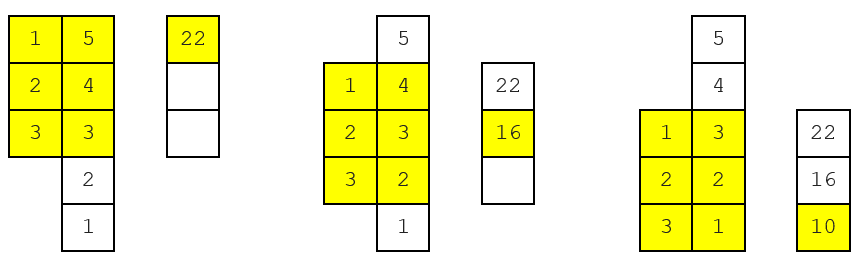
\includegraphics[width=0.5\paperwidth]{C:/Users/Admin/Desktop/Github/question_bank/LyX/static/img/9597-DHS-2018-P1-Q4-1}
\par\end{center}

Write program code to implement the convolution process for vectors.
Display the result to the screen.

\subsection*{Evidence 23 }

Program code. \hfill{}{[}5{]}

\subsection*{Evidence 24 }

Screenshot.\hfill{} {[}1{]}

\subsection*{Task 4.3 }

An example of the inner product for a matrix (2D array) is as follows:
\begin{center}
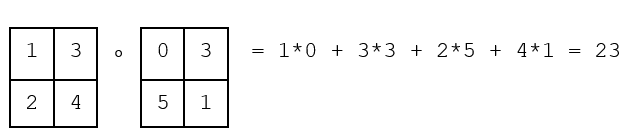
\includegraphics[width=0.5\paperwidth]{C:/Users/Admin/Desktop/Github/question_bank/LyX/static/img/9597-DHS-2018-P1-Q4-2}
\par\end{center}

Write program code to implement the convolution process for matrices
which uses the dot product for matrices. An example is shown below.
Display the result to the screen.
\begin{center}
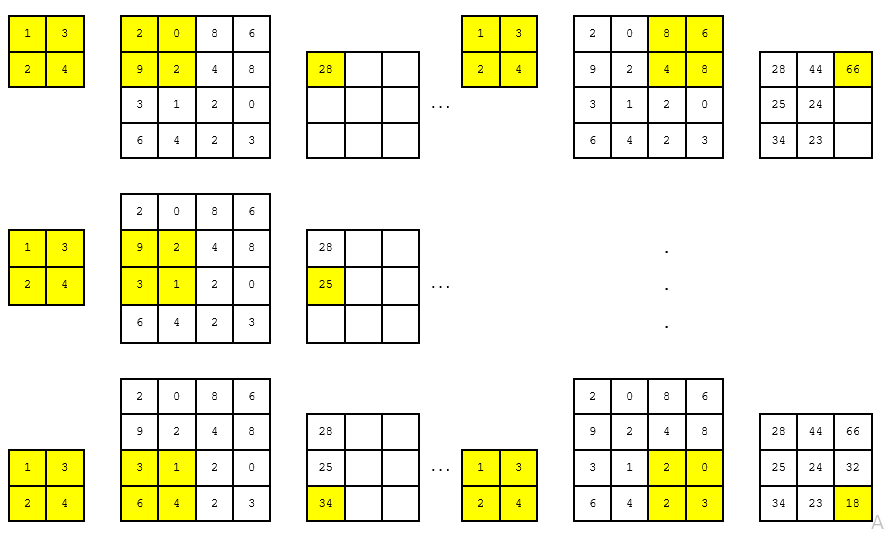
\includegraphics[width=0.65\paperwidth]{C:/Users/Admin/Desktop/Github/question_bank/LyX/static/img/9597-DHS-2018-P1-Q4-3}
\par\end{center}

\subsection*{Evidence 25 }

Program code. \hfill{}{[}8{]}

\subsection*{Evidence 26}

Screenshot.\hfill{} {[}2{]}

{[}SPLIT\_HERE{]}
\item \textbf{{[}DHS/PRELIM/9597/2018/P2/Q1{]} }

The Singapore Quick Response Code (SGQR) is a single QR code that
combines multiple e-payment solutions into one. It is intended to
simplify QR e-payments in Singapore for both consumers and merchants.

Currently, consumers see multiple QR codes at merchant stores promoting
various e-payment solutions. This can be confusing for consumers who
have to manually find if their preferred e-payment option is accepted.
Merchants are also impacted by the aesthetic and logistics constraints
of supporting multiple QR codes on their limited display and retail
space. With SGQR, consumers will see a single SGQR label that shows
all QR payment options that the merchant accepts. For merchants, SGQR
will be an infrastructure-light and cheaper way to accept multiple
types of e-payments.
\begin{center}

\includegraphics[width=0.25\paperwidth]{C:/Users/Admin/Desktop/Github/question_bank/LyX/static/img/9597-DHS-2018-P2-Q1}
\par\end{center}

Merchants that currently offer QR code payments will have their existing
QR codes replaced with a single SGQR label over the next six months.
The first phase of SGQR label replacement, starting with merchants
in the Central Business District, will be commencing in late September
2018.
\begin{enumerate}
\item You have been engaged as a project manager to oversee the implementation
of SGQR in Dunman High School (DHS) canteen. Produce a project proposal
outlining the key activities to make DHS canteen cashless by March
2019. Your proposal should include the essential elements such as
problem statement, project management processes and tools (e.g. PERT
chart and Gantt chart), roles of team members, etc. \hfill{}{[}19{]}
\item Beyond SGQR and in line with the Smart Nation drive, you have also
engaged a systems analyst to come up with an online food ordering
application to allow students and staff to avoid long queues and streamline
the food preparation process using their mobile devices. The school
management also wishes to keep track of the situation to provide feedback
to the canteen vendors. 

Outline the deliverables in the various phases of the software development
life cycle (specification, design, development, documentation, implementation,
testing/modification and maintenance). Be sure to adapt your answer
to the question context. \hfill{}{[}12{]}
\item Networking is critical in such a project/system. Give an example of
where each of the following networking concept is applicable in your
project/system.
\begin{enumerate}
\item synchronous and asynchronous data transmission
\item simplex, half duplex and full duplex mode of data transmission
\item packet switching and circuit switching for data transmission \hfill{}{[}6{]}
\end{enumerate}
\item You are also mindful about and is determined to prevent cybersecurity
attacks like the recent SingHealth data breach of the personal information
of 1.5 million patients. Outline a comprehensive organisational security
plan which goes beyond technical controls (user authentication, access
levels, antivirus, firewalls) to ensure that both the hardware infrastructure
and software applications are well secured against cybersecurity hacks.\hfill{}
{[}8{]}
\end{enumerate}
{[}SPLIT\_HERE{]}
\item \textbf{{[}DHS/PRELIM/9597/2018/P2/Q2{]} }

Mergesort uses a divide and conquer approach to successively divide
a list into half, forming two sublists, until each sublist is of length
1. The sublists are then sorted and merged into larger sublists until
they are recombined into a single sorted list. An algorithm for mergesort
is given below.

\noindent %
\noindent\begin{minipage}[t]{1\columnwidth}%
\texttt{procedure mergesort(mergelist)}

\texttt{\qquad{}if len(mergelist) > 1 then }

\texttt{\qquad{}\qquad{}mid = len(mergelist) div 2}

\texttt{\qquad{}\qquad{}lefthalf = mergelist{[}:mid{]}}

\texttt{\qquad{}\qquad{}righthalf = mergerlist{[}mid:{]}}

\texttt{\bigskip{}
}

\texttt{\qquad{}\qquad{}mergesort(lefthalf) }

\texttt{\qquad{}\qquad{}mergesort(righthalf)}

\texttt{\bigskip{}
}

\texttt{\qquad{}\qquad{}i = 0}

\texttt{\qquad{}\qquad{}j = 0}

\texttt{\qquad{}\qquad{}k = 0 }

\texttt{\qquad{}\qquad{}while i < len(lefthalf) and i < len(righthalf)}

\texttt{\qquad{}\qquad{}\qquad{}if lefthalf{[}i{]} < righthalf{[}j{]}
then}

\texttt{\qquad{}\qquad{}\qquad{}\qquad{}mergelist{[}k{]} = lefthalf{[}i{]}}

\texttt{\qquad{}\qquad{}\qquad{}\qquad{}i = i + 1 }

\texttt{\qquad{}\qquad{}\qquad{}else}

\texttt{\qquad{}\qquad{}\qquad{}\qquad{}mergelist{[}k{]} = righthalf{[}j{]} }

\texttt{\qquad{}\qquad{}\qquad{}\qquad{}j = j + 1}

\texttt{\qquad{}\qquad{}\qquad{}endif }

\texttt{\qquad{}\qquad{}\qquad{}k = k + 1 }

\texttt{\qquad{}\qquad{}endwhile }

\texttt{\bigskip{}
}

\texttt{\qquad{}\qquad{}while i < len(lefthalf) }

\texttt{\qquad{}\qquad{}\qquad{}mergelist{[}k{]} = lefthalf{[}i{]}}

\texttt{\qquad{}\qquad{}\qquad{}i = i + 1}

\texttt{\qquad{}\qquad{}\qquad{}k = k + 1 }

\texttt{\qquad{}\qquad{}endwhile}

\texttt{\qquad{}\qquad{}while j < len(righthalf)}

\texttt{\qquad{}\qquad{}\qquad{}mergelist{[}k{]} = righthalf{[}j{]}}

\texttt{\qquad{}\qquad{}\qquad{}j = j + 1}

\texttt{\qquad{}\qquad{}\qquad{}k = k + 1 }

\texttt{\qquad{}\qquad{}endwhile}

\texttt{\qquad{}endif }

\texttt{endprocedure}%
\end{minipage}
\begin{enumerate}
\item The following list of numbers is to be sorted using mergesort:

\texttt{mergelist = {[}5, 3, 2, 7, 9, 1, 3, 8{]}}

What are the first two lists to be merged? \hfill{}{[}2{]}
\item Draw a graphical representation of how the above list is first split
into halves until each sublist contains zero or one items, and then
the sublists are merged to become the sorted list. \hfill{}{[}4{]}
\item Give and justify the time complexity of mergesort. \hfill{}{[}2{]}
\item Compare the space complexities of mergesort and quicksort.\hfill{}
{[}2{]}
\end{enumerate}
{[}SPLIT\_HERE{]}
\item \textbf{{[}DHS/PRELIM/9597/2018/P2/Q3{]} }
\begin{enumerate}
\item Devise an algorithm to sort a list of words so that the anagrams are
grouped together.

For example, if the unsorted list is 

tar, phone, rat

after sorting we should get

tar, rat, phone

since tar and rat are anagrams, they are grouped together.\hfill{}{[}5{]}
\item Devise an algorithm to find the length of the longest palindrome in
a string s. \hfill{}{[}5{]}
\end{enumerate}
{[}SPLIT\_HERE{]}
\item \textbf{{[}DHS/PRELIM/9597/2018/P2/Q4{]} }

A program needs to be written to store and manage product information.
The program will have the following functionality:
\begin{itemize}
\item able to display a list of products in alphabetical order 
\item able to support efficient additions and deletions 
\item able to search for a product efficiently
\end{itemize}
\begin{enumerate}
\item Explain why it is better to use a binary search tree (BST) than an
ordered array to store and manage product information\hfill{}. {[}2{]}

The initial list of products to be stored are: 
\noindent \begin{center}
battery, cable, detergent, medicine, soap, towel, yoyo
\par\end{center}
\item Draw the BST 
\begin{enumerate}
\item from the initial list to support efficient seach, addition and deletion 
\item when new items earphone and eraser have been inserted in that order
\item when medicine has been deleted \hfill{}{[}5{]}
\end{enumerate}
\item State the postorder traversal output of the updated BST. \hfill{}{[}1{]}
\item Outline how the BST can be reorganised after a series of additions
and deletions to ensure optimal search performance.\hfill{} {[}2{]}
\end{enumerate}
{[}SPLIT\_HERE{]}
\item \textbf{{[}DHS/PRELIM/9597/2018/P2/Q5{]} }

A digital media company currently sells electronic books and audio
books. Each book has a unique id, title, image and price. An electronic
book has a default number of pages while an audio book has a duration. 
\begin{enumerate}
\item Draw a class diagram showing the relationship between the different
digital book types. \hfill{}{[}3{]}
\item Using appropriate examples, explain the following terms:
\begin{enumerate}
\item encapsulation
\item inheritance
\item polymorphism\hfill{} {[}6{]}
\end{enumerate}
\item To improve sales, the company decides to
\begin{enumerate}
\item Offer discounts on selected book items. Discounts on each book may
vary from 0 to 50\%.
\item sell digital movies. Each movie has a duration as well as a rating
with possible values G, PG and PG13. 
\item offer a monthly subscription service with unlimited access to all
digital media.
\end{enumerate}
Explain how these changes will affect your design in \textbf{part
(a)}. \hfill{}{[}6{]}
\end{enumerate}
{[}SPLIT\_HERE{]}
\item \textbf{{[}DHS/PRELIM/9597/2018/P2/Q6{]} }

The following figure shows the partial contents of an unnormalised
relational database table for library book loans by an amateur database
administrator. 
\noindent \begin{center}
\begin{tabular}{|c|c|c|c|c|c|c|c|c|}
\hline 
CallNo & Title & Author & PublisherID & PublisherName & BorrowerID & BorrowerName & Email & LoanDate\tabularnewline
\hline 
A2345 & Superhuman & Peter Smith & P0928 & Healthy Global & X894 & Robert Lim & roblim@gmail.com & 20181004\tabularnewline
\hline 
A1133 & Agile Methodology & Sophia Jones & P7823 & CS Books & X894 & Robert Lim & roblim@gmail.com & 20181004\tabularnewline
\hline 
B5104 & Python Advanced & Zen Wang & P8246 & Make It Harder & Y532 & Mary Tan & maryt@yahoo.com & 20181007\tabularnewline
\hline 
A2257 & Computer Science & Berry Mile & P8246 & Make It Harder & X451 & Ben Neo & benn@gmail.com & 20181007\tabularnewline
\hline 
B7513 & Alibaba & Jacky Ma & P3245 & Ali Pub  & X451 & Ben Neo & benn@gmail.com & 20181007\tabularnewline
\hline 
\end{tabular}
\par\end{center}

\begin{enumerate}
\item Give \textbf{two} potential anomalies that can occur with this design.
\hfill{}{[}2{]}
\item Give \textbf{two} advantages of normalisation. \hfill{}{[}2{]}
\item Give the table specification in 
\begin{enumerate}
\item 1NF
\item 2NF
\item 3NF \hfill{}{[}6{]}
\end{enumerate}
\item Draw an E-R diagram to represent your normalised design.\hfill{}
{[}3{]}
\item The following figure shows the notification email sent to the borrower
upon successful loan of library books.

\noindent\fbox{\begin{minipage}[t]{1\columnwidth - 2\fboxsep - 2\fboxrule}%
\texttt{Oct 4, 2018, 6:52 PM }

\texttt{From: NLB <helpdesk@nlb.gov.sg> }

\texttt{To: roblim@gmail.com}

\bigskip{}

\texttt{Dear Robert Lim}

\bigskip{}

\texttt{Thank you for using NLB's e-notification service through email,
a free service available to all library members.}

\bigskip{}

\texttt{This notification service confirms the number of items you
have borrowed at the library book borrowing station.}

\bigskip{}

\texttt{You have borrowed 2 item(s) at 18:52 on 4 Oct 2018 at Serangoon
Public Library:}

\bigskip{}

\texttt{1. Superhuman }

\texttt{~~~Due on: 25 October 2018}

\bigskip{}

\texttt{2. Agile Methodology }

\texttt{~~~Due on: 25 October 2018}

\bigskip{}

\texttt{You may also check your updated account status at http://www.nlb.gov.sg}%
\end{minipage}}

Describe how the customised contents of the notification email are
generated from the database. You may assume that the default loan
period is 21 days.\hfill{} {[}3{]}
\end{enumerate}
{[}SPLIT\_HERE{]}
\end{enumerate}
 
\end{document}
